\documentclass{beamer}

\usepackage[english]{babel}
\usepackage[T1]{fontenc}
\usepackage[utf8]{inputenc}

\usepackage{amsmath}	% math fonts
\usepackage{amsthm}
\usepackage{amsfonts}
\usepackage{amssymb}
\usepackage{marvosym}
\usepackage{mathtools}
\usepackage[SCI,RGB]{aaltologo}
\usepackage{natbib}
\usepackage{booktabs}
\usepackage{multicol}
\usepackage{pifont}
\usepackage{tabularx}
\newcolumntype{Y}{>{\centering\arraybackslash\setlength{\baselineskip}{2\baselineskip}}X}
\usepackage{multirow}


\usepackage[figurename=Fig.]{caption}

\usetheme{Sharelatex}
\usepackage[orientation=landscape,size=a0,scale=1.2]{beamerposter}
\setbeamertemplate{caption}[numbered]

%% Author and title information
\title{%
    Probabilistic framework for integration of mass spectrum and retention time information in small molecule identification
}
    
\author[\Letter: eric.bach@aalto.fi]{ % address for correspondence 
    Eric Bach\,$^{\text{1,\Letter}}$, %
    Simon Rogers\,$^{\text{2}}$,    %
    John Williamson\,$^{\text{2}}$,  %
    and Juho Rousu\,$^{\text{1}}$
}
    
\institute[]{%
    $^{\text{1}}$Helsinki institute for Information Technology (HIIT), Department of Computer Science, Aalto University, Espoo, Finland\\
    $^{\text{2}}$School of Computing Science, University of Glasgow, Glasgow, UK
}
    
\date{\today}
%%%%%%%%%%%%%%%%%%%%%%%%%%%%%%

%% Notation
\newcommand{\ms}{MS}
\newcommand{\lc}{LC}
\newcommand{\msone}{\ms$^1$}
\newcommand{\msms}{\ms$^2$}
\newcommand{\lcms}{\lc-\ms}
\newcommand{\lcmsms}{\lc-\msms}

\newcommand{\spec}{x}
\newcommand{\rt}{t}
\newcommand{\cands}{\mathcal{C}}
\newcommand{\seqlength}{N}
\DeclareMathOperator{\sign}{sign}

%% Commands
\newcommand{\todocite}{\textcolor{red}{\textbf{[CITATION]}}}
\newcommand{\cmark}{\textcolor{aaltoGreen}{\ding{51}}}
\newcommand{\xmark}{\textcolor{aaltoRed}{\ding{55}}}
\newcommand{\pmark}{\textcolor{aaltoOrange}{\ding{108}}}

%%%%%%%%%%%%%%%%%%%%%%%%%%%%%%
 


\mathtoolsset{showonlyrefs=true}


\begin{document}
\begin{frame}{}

\vfill
  
\begin{columns}[T]

\column{.32\linewidth}
    \begin{block}{{\normalsize 1. Small Molecule Identification in Untargeted Metabolomics}}
    \begin{itemize}
        \item Challenge in untargeted metabolomics studies: \textbf{Identification of the small molecules} present in a biological sample
        \item \textbf{\lcms$^\mathbf{2}$} widely used analysis platform: Liquid chromatography (LC) coupled with tandem mass spectrometry (\msms) (Fig.~\ref{fig:lcmsms_pipeline})
        \item Most machine learning approaches for small molecule identification only utilize \msms{} information \cite{Duehrkop2019, Brouard_ismb_2016}
        \item \lc{} retention time (RT) information can aid small molecule identification \cite{Ruttkies2016,Stanstrup2015}
        \item \textbf{Challenges utilizing RT information:} (1) \lc-system specific RTs and (2) public RT databases are limited in size and molecule coverage
    \end{itemize}
    \vspace{0.25cm}
    \begin{figure}[h]
        \centering
        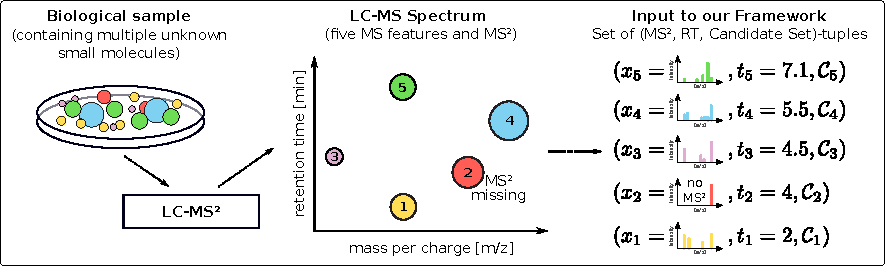
\includegraphics[width=\textwidth]{images/lcms2_experiment.pdf}
        \caption{\lcmsms{} analysis pipeline and resulting data used as input for our framework.}
        \label{fig:lcmsms_pipeline}
    \end{figure}
    \vspace{-0.75cm}
    \end{block}

    \begin{block}{{\normalsize 2. Retention Time (RT) Utilization for Small Molecule Identification}}
    \begin{itemize}
%         \item Multiple approaches in the literature to utilize RTs for molecule identification:
        \item[1)] \textbf{Comparison of measured RTs with (in-house) reference RTs}
        \item[$\circ$] References databases (DB) typically small and \lc-system specific
        \item[$\circ$] RT mapping between \lc-systems possible, but requires DB overlaps \cite{Stanstrup2015}
        \item[2)] \textbf{Comparison of measured RTs with predicted ones} \cite{Aicheler2015}  
        \item[$\circ$] RT prediction models allow to get RTs for practically every molecular structure
        \item[$\circ$] Majority of prediction models trained for a single \lc-system only
        \item[3)] \textbf{Compare RT-proxy or retention order with observed RT information} \cite{Ruttkies2016, Bach2018}
        \item[$\circ$] Allows for predictions within an whole \lc-system family, e.g. reversed-phase
        \item[$\circ$] Retention orders largely preserved across \lc-setups and prediction possible 
    \end{itemize}
    \vspace{0.25cm}
    \textcolor{red}{\bf Our proposed approach:}
    \begin{itemize}
        \item[\textcolor{red}{$\bullet$}] Exploitation of all pairwise observed retention orders in an \lcmsms{} datasets
        \item[\textcolor{red}{$\bullet$}] Comparison of observed and predicted retention orders to down- and up-vote potential molecular structures of the unknown molecules.
    \end{itemize}

    \end{block}

    \begin{block}{{\normalsize 3. \lcms$^\mathbf{2}$ Experiment Data: Input and Output of our Framework}}
    \begin{itemize}
        \item \textbf{Input:} Preprocessed \lcmsms{} data, i.e. after peak-picking and alignment (Fig.\ref{fig:lcmsms_pipeline}):
        \vspace{0.15cm}
            \begin{equation}
                \mathcal{D}=\{(\spec_i,\rt_i,\cands_i)\}_{i=1}^\seqlength
            \end{equation}
        \begin{tabularx}{\textwidth}{ccX}
            $\spec_i$ & : & \ms{} Information; \msms{}, or \msone{} (precursor m/z) if no fragmentation available \\
            $\rt_i$ & : & Measured RT \\
            $\cands_i$ & : & {Molecular candidate sets, e.g. molecular structures found in PubChem by \newline exact mass search} \\
            $\seqlength$ & : & Number of \ms{} features   \\
        \end{tabularx}
        \item \textbf{Precomputed \ms{} scoring assumed:} \msms{} scores, e.g. by CSI:FingerID \cite{Duehrkop2019}, MetFrag \cite{Ruttkies2016} or IOKR \cite{Brouard_ismb_2016}, or deviation of candidate and precursor mass for \msone{}
        \item \textbf{Output:} Ranking of the molecular candidates in $m_{ir}\in\mathcal{C}_i$ for each \ms{} feature $i$
        \item Ranking based on \ms{} and RT information
    \end{itemize}
    \vspace{-0.35cm}
    \end{block}

% ... end of first column

\hfill
\column{.34\linewidth}
    \begin{block}{{\normalsize 4. Probabilistic Framework to integrate \ms{} and RT Information}}
    \begin{itemize}
        \item \textbf{Graphical model} $G$ superimposed on the \lcmsms{} data (Fig.~\ref{fig:mrf_and_ranking})
        \item Let $G=(V,E)$ be complete graph with a \textbf{node} $i\in V$ for each \ms{} feature, and an \textbf{edge} $(i,j)\in E$ for each feature pair 
        \item Discrete random variable $z_i\in\mathcal{Z}_i=\{1,\ldots,n_i\}$ associated with each node ($n_i=|\cands_i|$)
        \item Candidate assignment for the complete data $\mathbf{z}=\{z_i\,|\,i\in V\}\in\mathcal{Z}_1\times\ldots\times\mathcal{Z}_\seqlength=\mathcal{Z}$
        \item Intuitively: Random variable $z_i$ denotes the candidate $m_{ir}\in\mathcal{C}_i$ assigned to feature $i$.
        \item Pairwise \textbf{Markov Random Field} as probabilistic model \cite{MacKay2005}:
            \begin{equation}
                p(\mathbf{z})=\frac{1}{Z}\prod_{i\in V}\psi_i(z_i)\prod_{(i,j)\in E}\psi_{ij}(z_i,z_j)
                \label{eq:mrf}
            \end{equation} 
        \item Potential functions: $\psi_i(z_i)$ \ms{} score and $\psi_{ij}(z_i,z_i)$ match of observed and \textbf{predicted retention order}
        \item Molecular \textbf{candidates ranked} based on max-marginals \cite{MacKay2005} (Fig.~\ref{fig:mrf_and_ranking}):
            \begin{equation}
                p_{\max}(z_i=r)=\underset{\{\mathbf{z}'\in\mathcal{Z}\,|\,z'_i=r\}}{\max}p(\mathbf{z}')
            \end{equation}
        \item Intuitively: Maximum marginal probability of a candidate assignment $\mathbf{z}$ with $z_i=r$.
    \end{itemize}
    \vspace{0.25cm}
    \begin{figure}
        \centering
        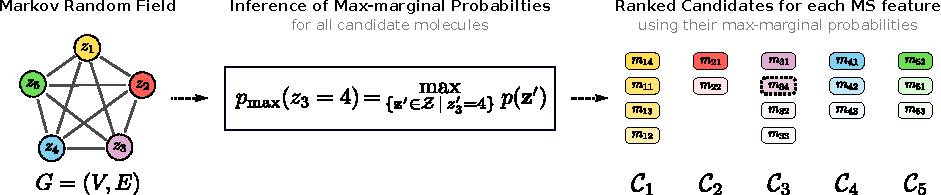
\includegraphics[width=\textwidth]{images/mrf_and_ranking.pdf}
        \caption{MRF probability distribution and candidate ranking, e.g. \ms{} feature $i=3$ and candidate $4$ ($m_{34}$).}
        \label{fig:mrf_and_ranking}
    \end{figure}
    \vspace{-0.75cm}
    \end{block}

    \begin{block}{{\normalsize 5. Encoding \ms{} and Retention Order Information: $\boldsymbol{\psi}_i$ and $\boldsymbol{\psi}_{ij}$}}
    \begin{itemize}
        \item Goodness of the candidate assignment $\mathbf{z}$ modeled by potential functions $\psi$ (Fig.~\ref{fig:node_and_edge_potentials})
        \item Node potential $\psi_i:\mathcal{Z}_i\rightarrow\mathbb{R}_{>0}$: $\psi_i(z_i=r)=f(x_i,m_{ir})$
        \item[$\circ$] $f$ returns the \ms{} matching score $\in(0,1]$ of spectrum $x_i$ and candidate $m_{ir}$
        \item Edge potential $\psi_{ij}:\mathcal{Z}_i\times\mathcal{Z}_j\rightarrow\mathbb{R}_{>0}$, with $\sigma$ being the sigmoid function:
            \begin{equation}
                \psi_{ij}(z_i=r,z_j=s)=\sigma(\underbrace{\sign(t_i-t_j)}_{\substack{\text{observed}\\ \text{retention order}}}\cdot\underbrace{\mathbf{w}^T(\phi(m_{ir})-\phi(m_{js}))}_{\text{predicted retention order}})
            \end{equation}
        \item Intuitively: Matching observed and predicted retention orders receive high scores.
        \item \textbf{Retention order prediction} using Ranking Support Vector Machine (RankSVM) $\mathbf{w}$ \cite{Bach2018}
        \item Candidate molecules $m_{ir}$ representation using non-linear features $\phi$ 
    \end{itemize}
    \vspace{0.25cm}
    \begin{figure}
        \centering
        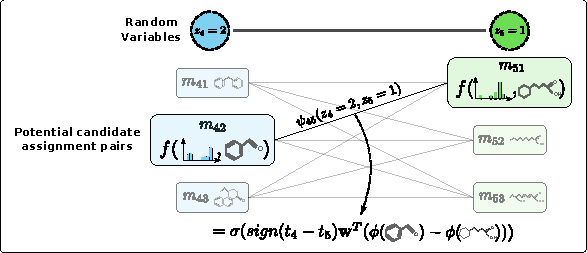
\includegraphics[width=0.8\textwidth]{images/node_and_edge_scores.pdf}
        \caption{Example: Node and edge score for all candidate pairs of feature $i=4$ and $j=5$.}
        \label{fig:node_and_edge_potentials}
    \end{figure}
    \vspace{-0.75cm}
    \end{block}


\hfill
\column{.32\linewidth} 

    \begin{block}{{\normalsize 6. Experiments and Results}}
    \begin{itemize}
        \item \textbf{Evaluation datasets:} CASMI 2016 \cite{Schymanski2017}, EA subset from MassBank used by \cite{Ruttkies2016} 
        \item[$\circ$] 681 (\msms, RT)-tuples with median number of candidates between 120 and 919
        \item[$\circ$] Datasets cover two different \lc{} columns and flow gradients
        \item \textbf{RankSVM training data:} 1248 RTs from PredRed \cite{Stanstrup2015} and CASMI 2016 training
        \item[$\circ$] No evaluation set molecule in RankSVM tranining set
        \item \textbf{Performance measure:} Top-$k$ accuracy, percentage of correct molecular candidates at rank $\leq k$
    \end{itemize}
    \vspace{0.5cm}
    \textbf{Experiment 1: Comparison to MetFrag + LogP (RT Proxy) Prediction}
    \begin{itemize}
        \item[$\circ$] MetFrag relaunched \cite{Ruttkies2016}: Prediction of LogP values for candidates, linear model mapping measured RTs to LogPs, candidate re-ranking based on LogP deviation
    \end{itemize}
        \begin{table}
            \centering
            \begin{tabular}{lcccc}
                \toprule
                \textbf{Method} & \textbf{Top-1} & \textbf{Top-5} & \textbf{Top-10} & \textbf{Top-20} \\ \midrule
                \msms{} + RT (Our) & 21.3 & 52.9 & 64.0 & 74.3 \\
                \msms{} + RT (MetFrag \& LogP) & 20.5 & 49.1 & 61.2 & 72.6 \\ \cmidrule(lr){1-5}
                Only \msms{} (baseline) & 16.7 & 49.5 & 60.4 & 70.6 \\
                \bottomrule
            \end{tabular}
        \end{table}
    \vspace{1cm}
    \textbf{Experiment 2: Performance with different \msms{}-Scoring Methods}
    \begin{itemize}
        \item[$\circ$] MetFrag (in-silico fragmenter scores) and IOKR \cite{Brouard_ismb_2016} as \msms{}-scoring methods
    \end{itemize}
        \begin{table}
            \centering
            \begin{tabular}{llcccc}
                \toprule
                {\bf \ms$^\mathbf{2}$-Scorer} & {\bf Method} & {\bf Top-1} & {\bf Top-5} & {\bf Top-10} & {\bf Top-20} \\ 
                \midrule
                    \multirow{2}{*}{MetFrag} &  \msms{} + RT (our) &   21.3 &   52.9 &    64.0 &    74.3 \\
                                             &  Only \msms{} (baseline) &   16.7 &   49.5 &    60.4 &    70.6 \\
                    \cmidrule(lr){1-6}
                    \multirow{2}{*}{IOKR} &  \msms{} + RT (our) &   26.7 &   52.1 &    62.5 &    70.3 \\
                                          &  Only \msms{} (baseline)&   25.1 &   49.5 &    60.3 &    67.6 \\
                \bottomrule
            \end{tabular}
        \end{table}
    \vspace{1cm}
    \textbf{Experiment 3: Missing \ms$^\mathbf{2}$ Spectra}
    \begin{itemize}
        \item[$\circ$] Simulating missing \msms{} information: Varying from 0\% to 100\% \msms
        \item[$\circ$] If only \msone{}: Use mass deviation between precursor and candidate molecule
    \end{itemize}
    \begin{figure}
        \centering
        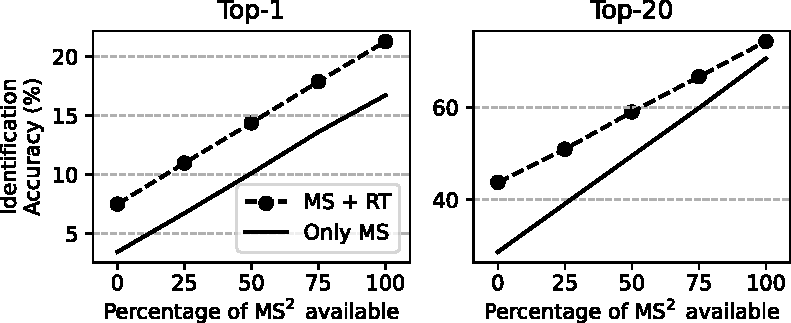
\includegraphics[width=0.7\textwidth]{images/missing_ms2.pdf}
    \end{figure}
    \vspace{-0.75cm}
    \end{block}

\vfill

\begin{block}{\small References}
    \bibliographystyle{abbrv}
    \vspace{-0.75cm}
    \begin{multicols}{2}
        \begin{footnotesize}
            \bibliography{biblib.bib}
        \end{footnotesize}
    \end{multicols} 
    \vspace{-0.35cm}
\end{block}
%% <== end of second column

\end{columns}

\vfill

\end{frame}
\end{document}
